
\chapter{Label System Design Considerations}
\label{ch:system-design}

Designing the labeling system supporting information flow tracking took special consideration.
FlowCore could have been written using one of two possible implementations of security types (Section~\ref{sec:implementation}): (1) extending of the tagged pointer representation and (2) introducing a security wrapper object.
Before choosing one implementation over the other, we first examine how each option affects the labeling of primitive values and interned objects and how the labeling mechanism will impact memory requirements (Section~\ref{sec:analysis}).
%We corroborate this analysis with a report on our experience during implementation (Section~\ref{sec:experience}).
Finally, we show how this work compares with that of others (Section~\ref{sec:related-work}), and finish with a recommendation that an extension of the tagged pointer representation meets the requirements of a dynamic information flow security type system and has the least implementation effort (Section~\ref{sec:conclusion}).

\section{Possible Implementations}
\label{sec:implementation}

Before discussing the details of the two possible implementations of dynamic security types, we first give a review of the existing dynamic type system that WebKit's JavaScriptCore VM employs.

\subsection{Existing Type System}

Many implementations of dynamically typed languages follow a common approach of using a tagged union to represent each possible primitive or object reference type~\cite{gudeman1993representing}.
In JavaScriptCore, this union takes the form of a 64-bit word, within the class \code{JSValue}.
Figure~\ref{fig:base-encoding} illustrates the union's fields as ordered on a big-endian\footnote{On a little-endian machine the order of the \code{tag} and \code{payload} fields are swapped.}, 64-bit machine.

\begin{comment}
   1  2   3      4
 0123456789abcdef
 0xffff ffff ffff ffff
    16   32        64

 signal nan:
 0x7ff0 0000 0000 0001 to
 0x7ff7 ffff ffff ffff
 or
 0xfff0 0000 0000 0001
 0xfff7 ffff ffff ffff

 quiet nan:
 0x7ff8 0000 0000 0001
 0x7fff ffff ffff ffff
 or
 0xfff8 0000 0000 0001
 0xffff ffff ffff ffff

 1 111 1 111 1 111 1---
 F     F     F     >8 

 E = 15 - 1 = 14 = 8 + 4 + 2
                   0111
                    - 1 // convert to actual double
                   0110 = 13
                   6

                   jsNan = 7ff8 0000 0000 0000
                           ffff                  tag type number
                           ----
                           true

                    jsNan -> asDouble
                    7ff8 0000 0000 0000
                -      1 0000 0000 0000       double encode offset
                   ---------------------
                    7ff7 0000 0000 0000       // now a signaling nan

\end{comment}

\begin{figure}[h!]
    \centering
\begin{tabular}{cc}
    \begin{minipage}[h]{.5\textwidth}
        \vfill
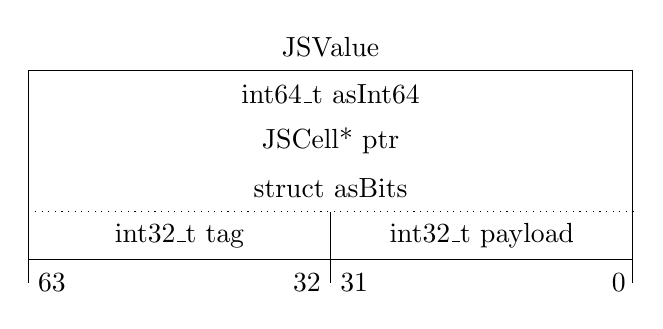
\begin{tikzpicture}[scale=.12]
 \draw[anchor=center] (32,2.5) node {\code{JSValue}};
 \draw (0,0) -- (0,-20) -- (64,-20) -- (64,0) -- cycle;
 \draw[anchor=center] (32,-2.5) node {\code{int64\_t asInt64}};
 %\draw[anchor=center] (32,-7.5) node {\code{double asDouble}};
 \draw[anchor=center] (32,-7.5) node {\code{JSCell* ptr}};
 %\draw (0,-10) -- (64,-10);
 \draw[anchor=center] (32,-12.5) node {\code{struct asBits}};
 \draw [dotted] (0,-15) -- (64,-15);
 \draw (32,-15) -- (32,-22.5);
 \draw[anchor=center] (16,-17.5) node {\code{int32\_t tag}};
 \draw[anchor=center] (48,-17.5) node {\code{int32\_t payload}};
 \draw (0,-20) -- (0,-22.5);
 \draw (64,-20) -- (64,-22.5);
 \node at (62.5,-22.5) {0};
 \node at (34.5,-22.5) {31};
 \node at (29.5,-22.5) {32};
 \node at (2.5,-22.5) {63};
\end{tikzpicture}
        \vfill
\end{minipage}
&
\begin{tabular}{c|l}
    bit values & type  \\
\hline
    \texttt{0000 0000 0000 0000} & \texttt{empty} \\
    \texttt{0000 0000 0000 0004} & \texttt{deleted} \\
    \texttt{0000 0000 0000 0002} & \texttt{null} \\
    \texttt{0000 0000 0000 0006} & \texttt{false} \\
    \texttt{0000 0000 0000 0007} & \texttt{true} \\
    \texttt{0000 0000 0000 000a} & \texttt{undefined} \\
    \texttt{0000 pppp pppp pppp} & \texttt{pointer} \\
    \texttt{0001 dddd dddd dddd} & \tikzmark{2nd} \multirow{3}{*}{\texttt{  double}} \\
    \texttt{\vdots} & \\
    \texttt{FFFE dddd dddd dddd} & \tikzmark{4th} \\
    \texttt{FFFF 0000 iiii iiii} & {integer}
\end{tabular}
\begin{tikzpicture}[overlay, remember picture]
    \draw [decoration={brace,amplitude=.5em}, decorate]
    ($(2nd)+(0,1ex)$) -- ($(4th)+(0,1ex)$);
\end{tikzpicture}

\end{tabular}
\caption{
    \label{fig:base-encoding}
    Representation of the internal \code{JSValue} class and the dynamic type encoding used in Webkit's JavaScriptCore VM.}
\end{figure}

\begin{comment}
         *     False:     0x06 =     4 + 2
         *     True:      0x07 =     4 + 2 + 1
         *     Undefined: 0x0a = 8     + 2
         *     Null:      0x02 =         2

         * These values have the following properties:
         * - Bit 1 (TagBitTypeOther) is set for all four values, allowing real pointers to be
         *   quickly distinguished from all immediate values, including these invalid pointers.
         * - With bit 3 is masked out (TagBitUndefined) Undefined and Null share the
         *   same value, allowing null & undefined to be quickly detected.
         *
         *     Deleted:   0x0
         *     Empty:   0x4
         * No valid JSValue will have the bit pattern 0x0, this is used to represent array
         * holes, and as a C++ 'no value' result (e.g. JSValue() has an internal value of 0).
        // These special values are never visible to JavaScript code; Empty is used to represent
        // Array holes, and for uninitialized JSValues. Deleted is used in hash table code.
        // These values would map to cell types in the JSValue encoding, but not valid GC cell
        // pointer should have either of these values (Empty is null, deleted is at an invalid
        // alignment for a GC cell, and in the zero page).
         */
\end{comment}


Within a \code{JSValue}, a leading value of \texttt{0xFFFF} distinguishes 32-bit JavaScript integers.
Doubles are offset (under bitwise integer interpretation) by the value $2^{48}$ to ensure that all values have at least a leading value of \texttt{0x0001}.
JavaScriptCore maintains a garbage collected heap which stores JavaScript objects with 64-bit alignment.
Pointers to garbage collected JavaScript objects all begin with a leading \texttt{0x0000}, which nominally reduces the address space to 48 bits\footnote{Modern 64-bit processors only supply 48 bits of addressable space, so JavaScriptCore's chosen pointer encoding does not reduce the actual usable space.}.
The special JavaScript values \code{null}, \code{false}, \code{true}, and \code{undefined} each have bit 1 set, to distinguish them from properly aligned pointer values.
JavaScriptCore also encodes two additional values, again at invalid pointer addresses, which are not defined within the JavaScript language: \code{empty}, which represents array holes and uninitialized \code{JSValue}s, and \code{deleted}, which is used in hash table code.


\subsection{Fat Value Technique}\label{sec:fat-values}
We can achieve dynamic information flow security by attaching, onto each runtime value, additional bits which encode a pointer, handle, or taint value representing the security type.
We term this technique the \term{fat value} approach, and extend the existing \code{JSValue} representation with an additional 64-bit word to hold the security type.
As shown in Figure~\ref{fig:fat-encoding}, each value within the interpreter then becomes 128-bits and contains both the originally encoded value and its security tag.

\begin{figure}[h]
\begin{minipage}[h]{.7\textwidth}
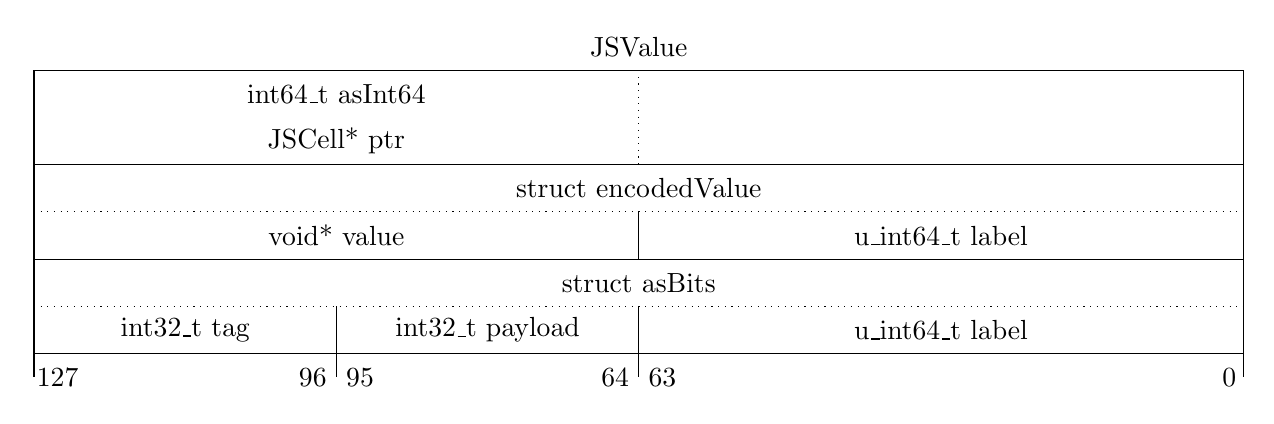
\begin{tikzpicture}[scale=.12]
 \begin{scope}[shift={(0,0)}]
 \draw (0,-5) rectangle (128,-15);
 \draw[anchor=center] (64,-2.5) node {\code{JSValue}};
 %\draw (64,-5) -- (64,-15);
 \draw[anchor=center] (32,-7.5) node {\code{int64\_t asInt64}};
 %\draw[anchor=center] (32,-12.5) node {\code{double asDouble}};
 \draw[anchor=center] (32,-12.5) node {\code{JSCell* ptr}};
 \draw[dotted] (64,-5) -- (64,-15);
 \end{scope}

 \begin{scope}[shift={(0,-15)}]
 \draw (0,0) rectangle (128,-10);
 \draw[dotted] (0,-5) -- (128,-5);
 \draw (64,-5) -- (64,-10);
 \draw[anchor=center] (64,-2.5) node {\code{struct encodedValue}};
 \draw[anchor=center] (32,-7.5) node {\code{void* value}};
 \draw[anchor=center] (96,-7.5) node {\code{u\_int64\_t label}};
 \end{scope}

 \begin{scope}[shift={(0,-25)}]
 \draw (0,0) rectangle (128,-10);
 \draw[anchor=center] (64,-2.5) node {\code{struct asBits}};
 \draw[dotted] (0,-5) -- (128,-5);
 \draw[anchor=center] (16,-7.5) node {\code{int32\_t tag}};
 \draw[anchor=center] (48,-7.5) node {\code{int32\_t payload}};
 \draw[anchor=center] (96,-7.5) node {\code{u\_int64\_t label}};
 \draw (32,-5) -- (32,-10);
 \draw (64,-5) -- (64,-10);
 \end{scope}

 \begin{scope}[shift={(0,-35)}]
 \draw (0,0) -- (0,-2.5);
 \node at (2.5,-2.5) {127};
 \node at (29.5,-2.5) {96};
 \draw (32,0) -- (32,-2.5);
 \node at (34.5,-2.5) {95};
 \node at (61.5,-2.5) {64};
 \draw (64,0) -- (64,-2.5);
 \node at (64+2.5,-2.5) {63};
 \node at (126.5,-2.5) {0};
 \draw (128,0) -- (128,-2.5);
 \end{scope}
\end{tikzpicture}
\end{minipage}
 \caption{Fat value encoding scheme.}
 \label{fig:fat-encoding}
\end{figure}\hfill

The fat value technique requires modifying the core representation of all values within the VM.
While performing this modification on an arbitrary dynamic language VM is not necessarily a trivial undertaking, the designers of JavaScriptCore have conveniently encapsulation the type inspection and conversion methods in the \code{JSValue} class.
This practice makes the modification easier than on other JavaScript VM's such as SpiderMonkey.
However, appropriately tagging each value with a security label still requires manual inspection of all code sites which create new values.
Additionally, doubling the size of the core datatype also doubles the memory space requirements of any running program: the VM allocates twice as much space for the same number of core values.

\subsection{Security Wrapper Technique}\label{sec:cloaks}

Another mechanism, known as the security wrapper technique, can also achieve the goal of attaching a security label to each value.
In this mechanism, the VM labels JavaScript objects by extending them with an additional internal field.
We introduce an internal security wrapper object which stores a primitive together with its label.
Throughout our analysis, we shall refer to this wrapper object as a \term{cloak} and any value held within the wrapper as a \term{cloaked} value.
Figure~\ref{fig:security-wrapper} provides a visualization of the cloak mechanism.

\begin{figure}[h]
 \centering
\begin{tikzpicture}[scale=.12]
    \node[anchor=center] at (12.5,2.5+2.5) {Object Reference};
    \node[anchor=center] at (12.5,2.5/2) {\tiny \texttt{0x0000 pppp pppp pppp}};
    \draw (0,0) rectangle (25,2.5);

    \coordinate (Obj) at (40,5);
    \node[anchor=center] at ($(Obj)+(15,2.5)$) {Cloak Object};
    \draw (Obj) rectangle ($(Obj)+(30,-15)$);
    \node[anchor=center] at ($(Obj)+(15,-2.5)$) {\vdots};
    \draw ($(Obj)-(0,5)$) -- ($(Obj)+(30,-5)$);
    \node[anchor=center] at ($(Obj)+(15,-5-2.5)$) {security label};
    \draw ($(Obj)-(0,10)$) -- ($(Obj)+(30,-10)$);
    \node[anchor=center] at ($(Obj)+(15,-10-2.5)$) {primitive value};

    \draw[-latex] (25,2.5/2) .. controls (25+15/2,2.5) and (25+15/2,5) ..  (Obj);

\end{tikzpicture}
\caption{Security wrapper scheme.}
\label{fig:security-wrapper}
\end{figure}

Internally, JavaScriptCore already supports wrapper classes for Strings and Dates, as well as automatic objection promotion for Numbers and Booleans.
Given this information, we might expect fewer modifications to be made to the underlying VM, as this change only requires the introduction of a new subclass of the existing \code{JSWrapperObject}.

However, implementing the wrapper class is not exactly trivial, even with the help of an existing framework.
From the perspective of the JavaScript program, a cloak object must mimic, in every circumstance, the same behavior as the primitive it cloaks.
Under no circumstances should the presence (or absence) of a security wrapper ever become evident to a JavaScript program, otherwise attacker provided code could exploit the difference in behavior.
%We make an exception to this guideline for policy violations, which have the side effect of halting the VM.
The wrapper must remain distinguishable to the VM, however, so that it can enforce information flow security.

Meeting this restriction is not presently possible using the existing wrapper framework.
The primary goals of the existing wrapper class is to collect those datatypes (Date, String, Number, and Boolean) which can be stored within the space of a \code{JSValue}.
As a result, the treatment of wrapped objects within the interpreter does not sufficiently take into account the behavioral differences between objects and primitives.
For example, in Listing~\ref{list:boolean}, a Boolean object wrapping the primitive value \code{false} behaves according to the rules governing objects rather than those of the primitive boolean value.
Consequently, the existing framework poses an imperfect fit for implementing information flow security, because it does not guarantee perfect transparency (from the perspective of a JavaScript program) when used to wrap primitives.

\lstset{caption={JavaScript considers objects as `truthy' values.},
        label={list:boolean}}
\begin{jscode}
js> var x = new Boolean(false)
js> if (x) { print("x is true"); }
    x is true
\end{jscode}

\section{Impacts on the Virtual Machine}
\label{sec:analysis}

Now that we have introduced two viable techniques for implementing information flow security, we analyze how each performs when labeling primitives, how each handles interned objects, and what impacts each has on memory requirements.
Although implementation details of JavaScriptCore serve as a guide, the following analysis applies to all other virtual machines that share the same design characteristics.

\subsection{Labeling Primitives}\label{sec:primitives}

%Although the tagged pointer encoding is an implementation detail, this decision has had side effects which have leaked into the JavaScript specification.
%The foundational JavaScript VM, SpiderMonkey, initially implemented a tagged pointer encoding scheme for the 32-bit machines of that era.
%For example, SpiderMonkey's original 32-bit implementation used 1 bit for the integer type tag, and 31 bits for integer values.
%This design forced the language specification~\cite{ecma} to provide a coercion of any integer which cannot be represented by 31-bits to the \texttt{double} type.

The existing core datatype in JavaScriptCore uses a NaN encoding scheme that enables the value and type tag to coexist in the same memory structure.
The tagged pointer technique has the benefit of allowing the VM to perform operations on primitives quickly and directly.
Unfortunately, many common operators, such as \texttt{+}, behave differently depending on the types of the arguments.
Not only must the VM first inspect the type of the core values involved before dispatching the operation, but it then also unpacks the payload of the arguments from their encoding.

Using the fat value approach requires modifying the core value representation, extending it with additional bits to hold the security type.
This modification impacts the mechanisms used to encode and decode primitive values, as well as the type inspection routines.
JavaScriptCore uses an Object-Oriented design that encapsulates the type inspection logic, preventing it from dispersing across the VM implementation.
However, we must still manually audit each site at which the VM creates \code{JSValue}s so that the appropriate security label can be set.

Alternatively, the cloak approach requires the creation of a wrapper object for each labeled primitive.
Although the cloak easily holds both the core value representation of the primitive as well as the security type, the presence of a cloak object negatively impacts the runtime type inspection logic.
Where before the VM would previously inspect a primitive, it now dispatches inspection logic on a cloak object.
This extra layer of indirection severely degrades the performance of the very operations for which primitives are optimized.

The WebKit developers have designed JavaScriptCore as an embeddable interpreter.
Systems external to the JavaScript engine, such as the DOM framework of the WebKit browser, reflect their own classes into the JavaScriptCore engine.
This reflection occurs via a layer of interface classes\footnote{The WebKit build system automatically generates the interface classes.}, which each inherit a JavaScriptCore class such as \code{JSNonFinalObject}.
Should an external system expect certain fields to contain raw primitives (such as integers), it will fail when receiving a cloaked value.
When implementing the cloak scheme, we must either prohibit cloaks from escaping the JavascriptCore VM or modify the interface layer to automatically uncloak.
Both of these solutions leave the browser's external systems open as an information side channel.

To avoid observable semantic changes that could be exploited by an attacker, cloaks must also remain completely invisible to the JavaScript programmer.
For example, even though we implement cloaks as a native \code{JSObject} within the VM, we cannot allow a JavaScript program to set a property on a cloaked primitive.
Additionally, some JavaScript operators, such as \code{typeof}, require introducing an additional special case.
For example, a cloaked integer reports the type of the cloaked value, ``\code{number}'', rather than the type of the cloak, ``\code{object}''.
Should the VM use this operator internally for a type dispatch, it would then pass the value into a native routine expecting a raw primitive value.
To reduce the amount of implementation effort, we seek to avoid hunting down all the type dispatch sites and introducing these special cases.

When we compare the fat value approach to the cloak approach, an interesting semantic difference arises:
In the fat value approach, we attach the security type to the primitive value or object reference, as part of the tagged pointer encoding.
In the cloak approach, each object receives an internal field to store its security label, while primitives are cloaked with an extra layer of indirection.

\todo{I haven’t fully explored the difference between having a labeled reference vs having a labeled object, but I think the difference is analogous to having an Access Control Listing by columns vs Object Capabilities by rows, as discussed in Capability Myths Demolished.}
% At this point I am in favor of the fat value approach, because I’m liking the reference semantics, and the transparency with which primitives can be labeled. I’m also willing to accept the cost of having fatter values.

\subsection{Interned Objects}\label{sec:interned-objects}

The JavaScriptCore VM employs optimizations pioneered by earlier dynamically typed languages, such as Lisp and Scheme.
To achieve better runtime performance and reduce memory footprint, the VM interns contents of type \code{string}.
Figure~\ref{list:intern} clarifies the terminology we use to differentiate the storage aspects of JavaScriptCore's interning optimization.
Semantically, JavaScriptCore separates primitive strings from string objects.
In order to permit the storage of properties, JavaScriptCore separately instantiates each string object, regardless of its contents.
To enable fast comparison, equality, and identity operations, the VM implements string primitives as pointers to internal \code{JSString} objects which hold the string contents.

\begin{figure}[h]
  \centerline{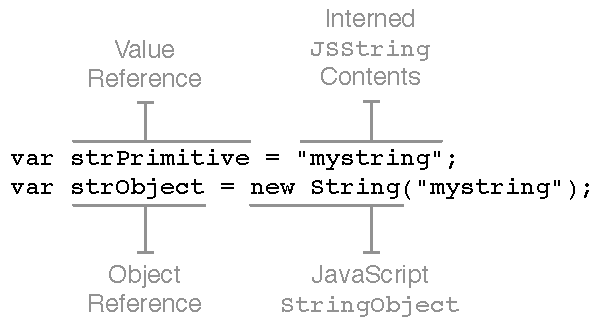
\includegraphics[keepaspectratio=true]{images/InternedTerminology.pdf}}
  \caption{Terminology used to describe interning.}
  \label{list:intern}
\end{figure}

Within an information flow framework, we need to record both the security context of creation as well as the contents of new objects and values.
Because the interning optimization allows two string primitives to reference the same interned string contents we must be careful about our placement of the information flow security labels.
Specifically, we seek to prevent the sharing of a label across two string primitives which happen to reference the same interned contents.

%As a side effect of interning, references to strings containing the same contents all point to the same string value.
In one possible scheme, we could place the security label on the interned string content.
This placement causes the label to be shared among all references.
Under this scheme, an attacker could manufacture a JavaScript function that returns a string primitive carrying an incorrect label (see Listing~\ref{list:interned-string}).

\lstset{caption={A function returning the value ``\code{String}'' which can carry one of two different security labels depending on runtime control flow.},
        label=list:interned-string}
\begin{jscode}
function foo(x) {
  var a = "mystring"    // This variable is interned with the
                        // same security label as the code for
                        // the function "foo".

  if (x) {              // The label of "b" needs to reflect
    var b = "mystring"  // a dependence on "x". It should not
  }                     // affect the label attached to "a".

  return a
}
\end{jscode}

One solution to this dilemma is to automatically upgrade the label attached to the interned string value.
However, this solution causes unnecessary upgrades, as each occurrence of the string will upgrade the attached security label, even when such occurrences are completely independent.
With each successive use of the interned string, the upgraded label propagates throughout the system, becoming a source of label creep.
This strategy propagates a false information flow dependence when completely separate and non-interfering code routines reference the same string contents purely as a side effect interning.
We observe from this approach that placing the security label on the \emph{referent} will not allow the information flow framework to distinguish the code paths and security contexts on which the \emph{reference} depends.

The cloak approach permits another solution, as it stores the label on the cloak object wrapping the primitive string.
We prefer this approach over the previous one, because it places the security label on the reference, allowing the information flow framework to differentiate primitives and objects from interned contents.
From the perspective of a JavaScript program, the semantics of cloaked primitive strings are now seen to obey the same rules as that of directly labeled references.

Interestingly, the fat value approach already provides such semantics.
No additional provisions need be made for the special case of interned objects, as all object references also carry a security label, by virtue of extending the tagged pointer representation.
Indeed, the fat value approach even saves computation access costs by avoiding the layer of indirection incurred by introducing cloak objects.

\subsection{Systemic Memory Impacts}\label{sec:garbage-collection}

Both the fat value and cloak approaches require supporting data structures, such as a runtime lattice of security labels, which add to the memory requirements of the system.
This memory overhead is the same for both approaches, so we do not consider it as part of the following analysis.

The cloak approach creates an entire object for each primitive value that requires labeling.
Creating these wrappers can drastically lower the performance of the overall system, stressing the garbage collector.
As a side-effect of label creep, cloaked values become more common than not.
Creating an object for each of these labeled values forces the garbage collector to spend much more time in both the mark and sweep phases.
The additional memory allocation calls required when creating cloak objects impacts most exactly that feature of JavaScript designed to be performant: primitives.

The fat value approach avoids these problems with the garbage collector by extending the representation of primitives and object references with additional bits to hold a security label.
However, this extension doubles the overall memory requirements of the system.
Both values placed in the function call stack and property fields within an object increase by the amount of space necessary for the attached label.
However, the memory overhead required by the security labels remains far less than the additional storage required when creating a cloak object.

\begin{comment}
memory overhead, cloak approach:
  1 cloak object per primitive = sizeof(jscloak) == jsfinalobject
  what about extending each object with an internal label field ? (can jsobject stay at 32 bytes?)
  [ putting a void* in jsobject: JSObject=8*5=40, JSFinalObject=8*9=72, JSNonFinalObject=8*7=56 ]
  [ does this change packing in the gc? it does affect compile asserts on storage size vptrs (JSGlobalData) ]
  
memory overhead, fat-value approach:
  2x number of JSValues in system

without jsflow (base):
COMPILE_ASSERT(sizeof(char) == 1, invalid_sizeof_char);
COMPILE_ASSERT(sizeof(void*) == 8, invalid_sizeof_void_ptr);
COMPILE_ASSERT(sizeof(JSObject) == 32, invalid_sizeof_jsobject);
COMPILE_ASSERT(sizeof(JSCell) == 16, invalid_sizeof_jscell);
COMPILE_ASSERT(sizeof(JSValue) == 8, invalid_sizeof_jsvalue);
COMPILE_ASSERT(sizeof(JSFinalObject) == 8*8, invalid_sizeof_jsfinalobject);
COMPILE_ASSERT(sizeof(JSNonFinalObject) == 8*6, invalid_sizeof_jsnonfinalobject);

with jsflow (fat-value):
COMPILE_ASSERT(sizeof(char) == 1, invalid_sizeof_char);
COMPILE_ASSERT(sizeof(void*) == 8, invalid_sizeof_void_ptr);
COMPILE_ASSERT(sizeof(JSObject) == 32, invalid_sizeof_jsobject);
COMPILE_ASSERT(sizeof(JSCell) == 16, invalid_sizeof_jscell);
COMPILE_ASSERT(sizeof(JSValue) == 16, invalid_sizeof_jsvalue);
COMPILE_ASSERT(sizeof(JSFinalObject) == 8*12, invalid_sizeof_jsfinalobject_12);
COMPILE_ASSERT(sizeof(JSNonFinalObject) == 8*8, invalid_sizeof_jsnonfinalobject);

#define JSNonFinalObject_inlineStorageCapacity 2
#define JSFinalObject_inlineStorageCapacity 4
\end{comment}

%\section{Implementation Experience}\label{sec:experience}

\begin{comment}
Previous outline:

* could only talk about cloaks implementation
- discovered primitives leaking to other systems (Alexa)
- had to explicitly label, couldn't optimize (operand stack and scope)
- abstract interpreter (correctness)

I don't have an implementation of the cloaks, only of fat-values.
For the fat-values only, I can generate precise timing measurements for each aspect of the system.
There isn't a big problem interfacing with other systems, as they get the jsvalue layout through header file, and ignore the label part.
Everything is explicitly labeled, no opportunity for memory optimization.
Have abstract interpreter for stack label alignment [probably want to mention in later section]
\end{comment}

\section{Summary}

Given our analysis (Section~\ref{sec:analysis}), we can now achieve a high-level overview of the two techniques for introducing security types in an existing interpreter.
Each technique features design trade-offs concerning development effort, runtime costs, and security enforcement.
%We discuss these trade-offs in the context of our implementation experience (Section~\ref{sec:experience}) with the SpiderMonkey JavaScript interpreter.

\subsection{Impacts on Implementation}
The fat value technique extends the tagged pointer representation of the core value type of the interpreter.
By embedding the security label into the core representation, the VM has fast and convenient access to the label on each piece of data involved in a computation.
In contrast, the cloak approach introduces a wrapper object which holds both the primitive value and the security label, requiring an additional step when accessing either the value or label.
Because the VM manipulates labels in many of the underlying opcodes and JavaScript programmers expect primitives to be performant, access to both the label and value should be kept as direct as possible.

The security labels constitute their own security type system, orthogonal to the existing JavaScript value types.
The fat value approach modifies the representation of the interpreter's core datatype to add labels.
The well-factored design of JavaScriptCore allows this modification to be made easily, without spending effort to manually inspect existing type-dispatch sites.

Although the cloak approach avoids changing the core datatype, it creates a wrapper object around primitive values that introduces an additional layer of indirection during type-dispatch operations.
Security constraints require cloak objects to override operators such as \code{typeof} so as to maintain invisibility from the perspective of a JavaScript program.
When operating on a cloaked primitive, the VM encounters and dispatches on the cloak object, which in turn inspects its contents and performs the operation on the wrapped primitive value.
This two-level dispatch puts cloaked primitives on a slow execution path during performance critical type-dispatch operations.

\medskip
\begin{figure}[h]
\centering
\resizebox{\columnwidth}{!}{
\begin{tabular}{l|l|l}
\toprule
\multicolumn{3}{c}{Impacts on Implementation} \\
\midrule
\multicolumn{1}{c}{Concern} & \multicolumn{1}{|c|}{Fat Values} & \multicolumn{1}{c}{Cloaks} \\
\midrule
Integration      & Modifies core datatype representation & Introduces new cloak object \\
Label Access     & Direct & Indirect \\
VM Type-Dispatch & Unaffected & Dispatched chained after VM \\
\bottomrule
\end{tabular}
}
\end{figure}
\medskip

\subsection{Impacts on the Runtime System}

Both the cloak and fat value techniques increase the memory size of running programs.
We focus our analysis only on the memory requirements which differ between these two techniques, and ignore memory increases, such as objects representing a label hierarchy or a runtime stack of security labels, which are common to both techniques.

By extending the core representation of all values, the fat value technique doubles the size of the core datatype, \code{JSValue}.
This increase extends to any \code{JSValue}s internally held by JavaScript classes such as \code{JSArray} and internal classes such as \code{RegisterFile}
The increase also extends to all dynamically assigned properties on JavaScript objects, roughly doubling the memory requirements of the entire VM.
In contrast, the cloak approach requires a single field be added to all objects, which the VM uses for security tagging, increasing memory requirements 20\% for each JavaScript object\footnote{On a 64-bit system, the unmodified \code{JSObject} base class requires 32 bytes. Introducing the label field requires 8 bytes, a 20\% increase. Other classes inheriting \code{JSObject} have a smaller percentage increase. For example, \code{JSNonFinalObject}, which abstracts most of JavaScript's built-in prototype objects, requires 48 bytes.}.
Additionally, the cloak class itself increases the memory requirements 600\% for each primitive\footnote{On a 64 bit system, primitive \code{JSValue}s are 8 bytes, while the \code{JSCloak} class requires 48 bytes, a 6x increase.}.

Technical difficulties of the JavaScriptCore design prevented implementation of sparse labeling~\cite{sparse-labeling} and forced conservative cloaking of primitive values.
Because of label creep, many primitives quickly require labeling, leading to the allocation of cloak objects.
The cloak technique only uses less memory than the fat value technique in situations where very few primitive values require labeling.
In our experience, this situation does not normally arise, because the VM labels values in many common operations, such as function returns and binary operations with at least one labeled argument.

Even worse, the allocation of a cloak object for each labeled primitive leads to much larger heap sizes, negatively affecting the performance of the garbage collector.
The fat value technique avoids this cost.
However, if the security implementation requires labels objects (pointed to by the label field of a fat value) then it needs a mechanism to indicate when a label object can be freed.
Because a label object remains alive only when it's pointed at by a live value, the garbage collector can be re-used to provide this feature\footnote{The VM could also use simple reference counting, as the label lattice contains no cycles.}.

Finally, the cloaking approach negatively impacts runtime performance more than the fat value technique, because cloaking places the label on an indirect path.
Each time the VM performs an operation, it typically labels the resulting value with the join of the labels of all arguments.
Keeping these labels directly accessible prevents an otherwise severe runtime overhead.
Additionally, JavaScript programmers expect operations on primitives to remain performant, so the extra dispatch needed to obtain the underlying primitive from a cloak negatively impacts performance in the least desirable manner.

\medskip
\begin{figure}[h]
\centering
\resizebox{\columnwidth}{!}{
\begin{tabular}{l|l|l}
\toprule
\multicolumn{3}{c}{Impacts on the Runtime System} \\
\midrule
\multicolumn{1}{c}{Concern} & \multicolumn{1}{|c|}{Fat Values} & \multicolumn{1}{c}{Cloaks} \\
\midrule
Memory Requirements & All core values double in size & Add internal label field to all objects \\
Object Allocation   & None, every core value carries a label & Only labeled primitives require a cloak object \\
Garbage Collection  & None, labels implemented as references  & Cloaked primitives require wrapper objects \\
Label Storage       & Optionally use GC to keep labels alive & Optionally use GC to keep labels alive \\
Runtime Speed       & All primitives stay on fast path & Cloaked primitives move to slow path \\
\bottomrule
\end{tabular}
}
\end{figure}
\medskip

\subsection{Impacts on Security Semantics}

As an embeddable language, JavaScript allows the host environment to expose functionality to the client programs.
For example, within the WebKit browser the DOM subsystem reflects native C++ objects into the JavaScriptCore VM.
Although it requires a re-compilation of the host's interface code, the fat value technique allows the host environment the freedom to ignore the label extension on core values.
In contrast, the cloak technique exports labeled primitives as cloak objects, leaking the security abstraction into the host environment.
Host interface code which expects a primitive value may fault when encountering a cloak object instead.
%We experienced exactly this problem when implementing cloaks in Firefox's JavaScript interpreter, SpiderMonkey.

The implementation differences between the cloak and fat value approaches extends beyond interaction with the host environment and imply different security semantics.
Not only is the label in a fat value optionally ignorable, but the direct attachment of a label to the core value creates a labeled reference semantics.
This semantics allows the VM to treat differently separate references to the same object, avoiding the confusion of identity that can result from having interned objects.
By attaching labels only to objects, the cloak approach provides a labeled object semantics.
Unfortunately, becasue of this attachment, the label of an object becomes shared among all references to that object.
As the object is used in different contexts, the attached label monotonically escalates, becoming a source of label creep.

\medskip
\begin{figure}[h]
\centering
\resizebox{\columnwidth}{!}{
\begin{tabular}{l|l|l}
\toprule
\multicolumn{3}{c}{Impacts on Security Semantics} \\
\midrule
\multicolumn{1}{c}{Concern} & \multicolumn{1}{|c|}{Fat Values} & \multicolumn{1}{c}{Cloaks} \\
\midrule
VM Abstraction Cost & VM can ignore security tag bits & Cloaks handled as special case \\
Host Abstraction Cost & Host can ignore security tag bits & VM must prevent leaking cloak objects \\
Security Semantics  & Labeled reference & Labeled value \\
\bottomrule
\end{tabular}
}
\end{figure}
\medskip

\section{Related Implementations}\label{sec:related-work}

\todo{rewriting approach of Jang}
\todo{DO: DOM interaction + channels}

\section{Chosen Implementation for FlowCore}\label{sec:conclusion}

Although both the fat value and cloak approaches can assist information flow security by adding runtime security types to all values within an existing dynamically typed language, this work uses the fat value approach, because it
(1) provides a reference semantics that works with interned objects,
(2) does not stress the garbage collector with unnecessary object creation,
and (3) easily labels every primitive and object reference.
Achieving these gains comes at the cost of:
(1) changing the representation of a core data type within the VM,
(2) auditing sites where type inspection occurs to ensure compliance with the new security system,
(3) extending all stack slots and object fields by the amount needed to store the security labels (a factor of 2).
These costs are worth the associated benefits, because the cloak approach:
(1) stresses the garbage collector adding runtime overhead unrelated to security enforcement,
(2) reduces performance by adding an additional layer of indirection,
(3) does not provide a conceptually uniform treatment of objects and primitives,
and (4) is more difficult to ensure invisibility from the perspective of the JavaScript programmer.

Interestingly, the performance optimizations, such as interning \code{string} objects, can have an adverse affect on security.
In particular, the interned object optimization confuses the issues of object identity and equality, in order to reduce the number of allocated objects and provide quick results for the string comparison operators.
In information flow security, the fact that two immutable objects might carry the same value implies nothing about their point of origin or the security actors which have influenced the object.
The labeled reference semantics provided by the fat value technique usefully allows distinguishing the security label of an object from the value of that object.
Fortunately, this semantics means that it is possible to keep the interned object optimization, even during implementing dynamic labeling for information flow security.

Given the difficulty and work involved during my implementation experience I wholeheartedly corroborate the statement: ``security is not a separable concern''\cite{miller2005structure}.


